\chapter{Benchmarking QUBO solvers}
\label{benchmark}

\section{Related benchmarking work}
Willsch et al.~\cite{b34} evaluated the performance of the QAOA algorithm and the D-Wave quantum annealer using instances of MaxCut and 2-satisfiability problems with up to 18 variables. The performance of the QAOA algorithm is inconsistent and underperforms quantum annealing in their problem set~\cite{b34}. 

Similarly, Pelofske et al.~\cite{b35} compared the performance of QAOA and quantum annealing on Ising models with cubic interaction terms and also found that quantum annealing had superior performance over QAOA. 

The benchmarking work of NNQS against other quantum-based QUBO solving methods is unexplored.

\section{Results}
Increase to 500 for classic solvers.

\subsection{NAE3SAT}
\begin{figure}[!h]
    \centering
    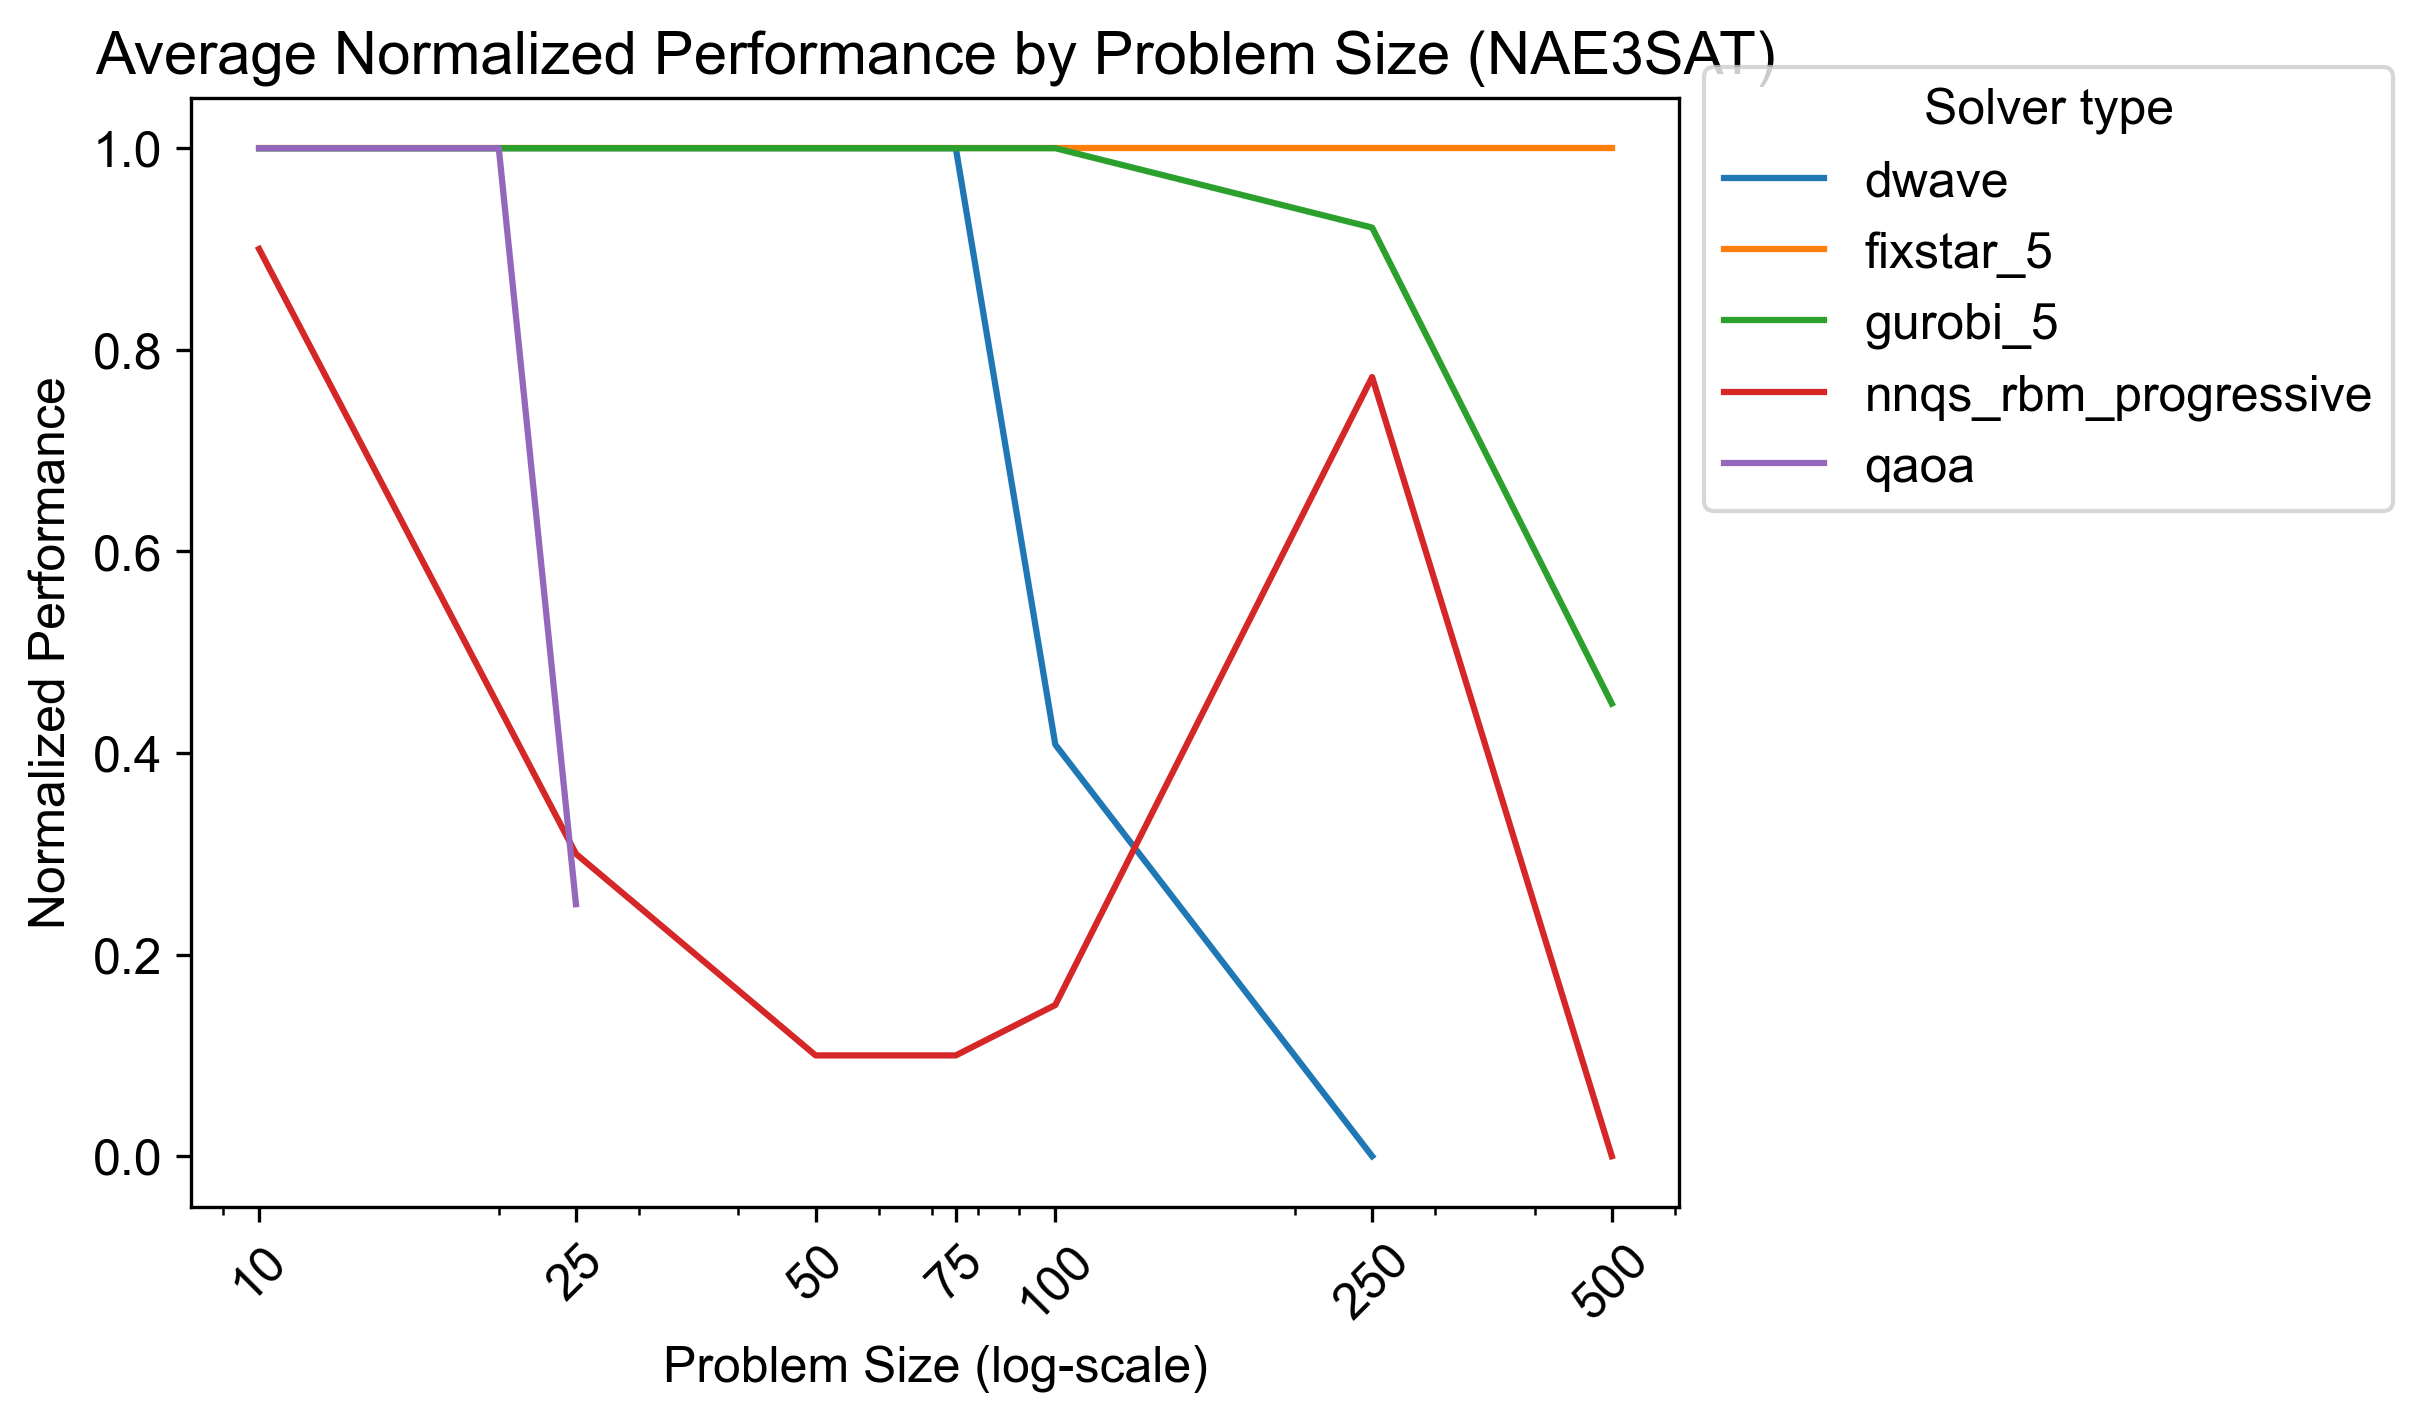
\includegraphics[width=1\linewidth]{images/nae3sat_normalized_performance_all.png}
    \caption{Normalized performance by size on the NAE3SAT dataset}
    \label{all-nae3sat-size}
\end{figure}

\subsection{Max-cut}
\begin{figure}[!h]
    \centering
    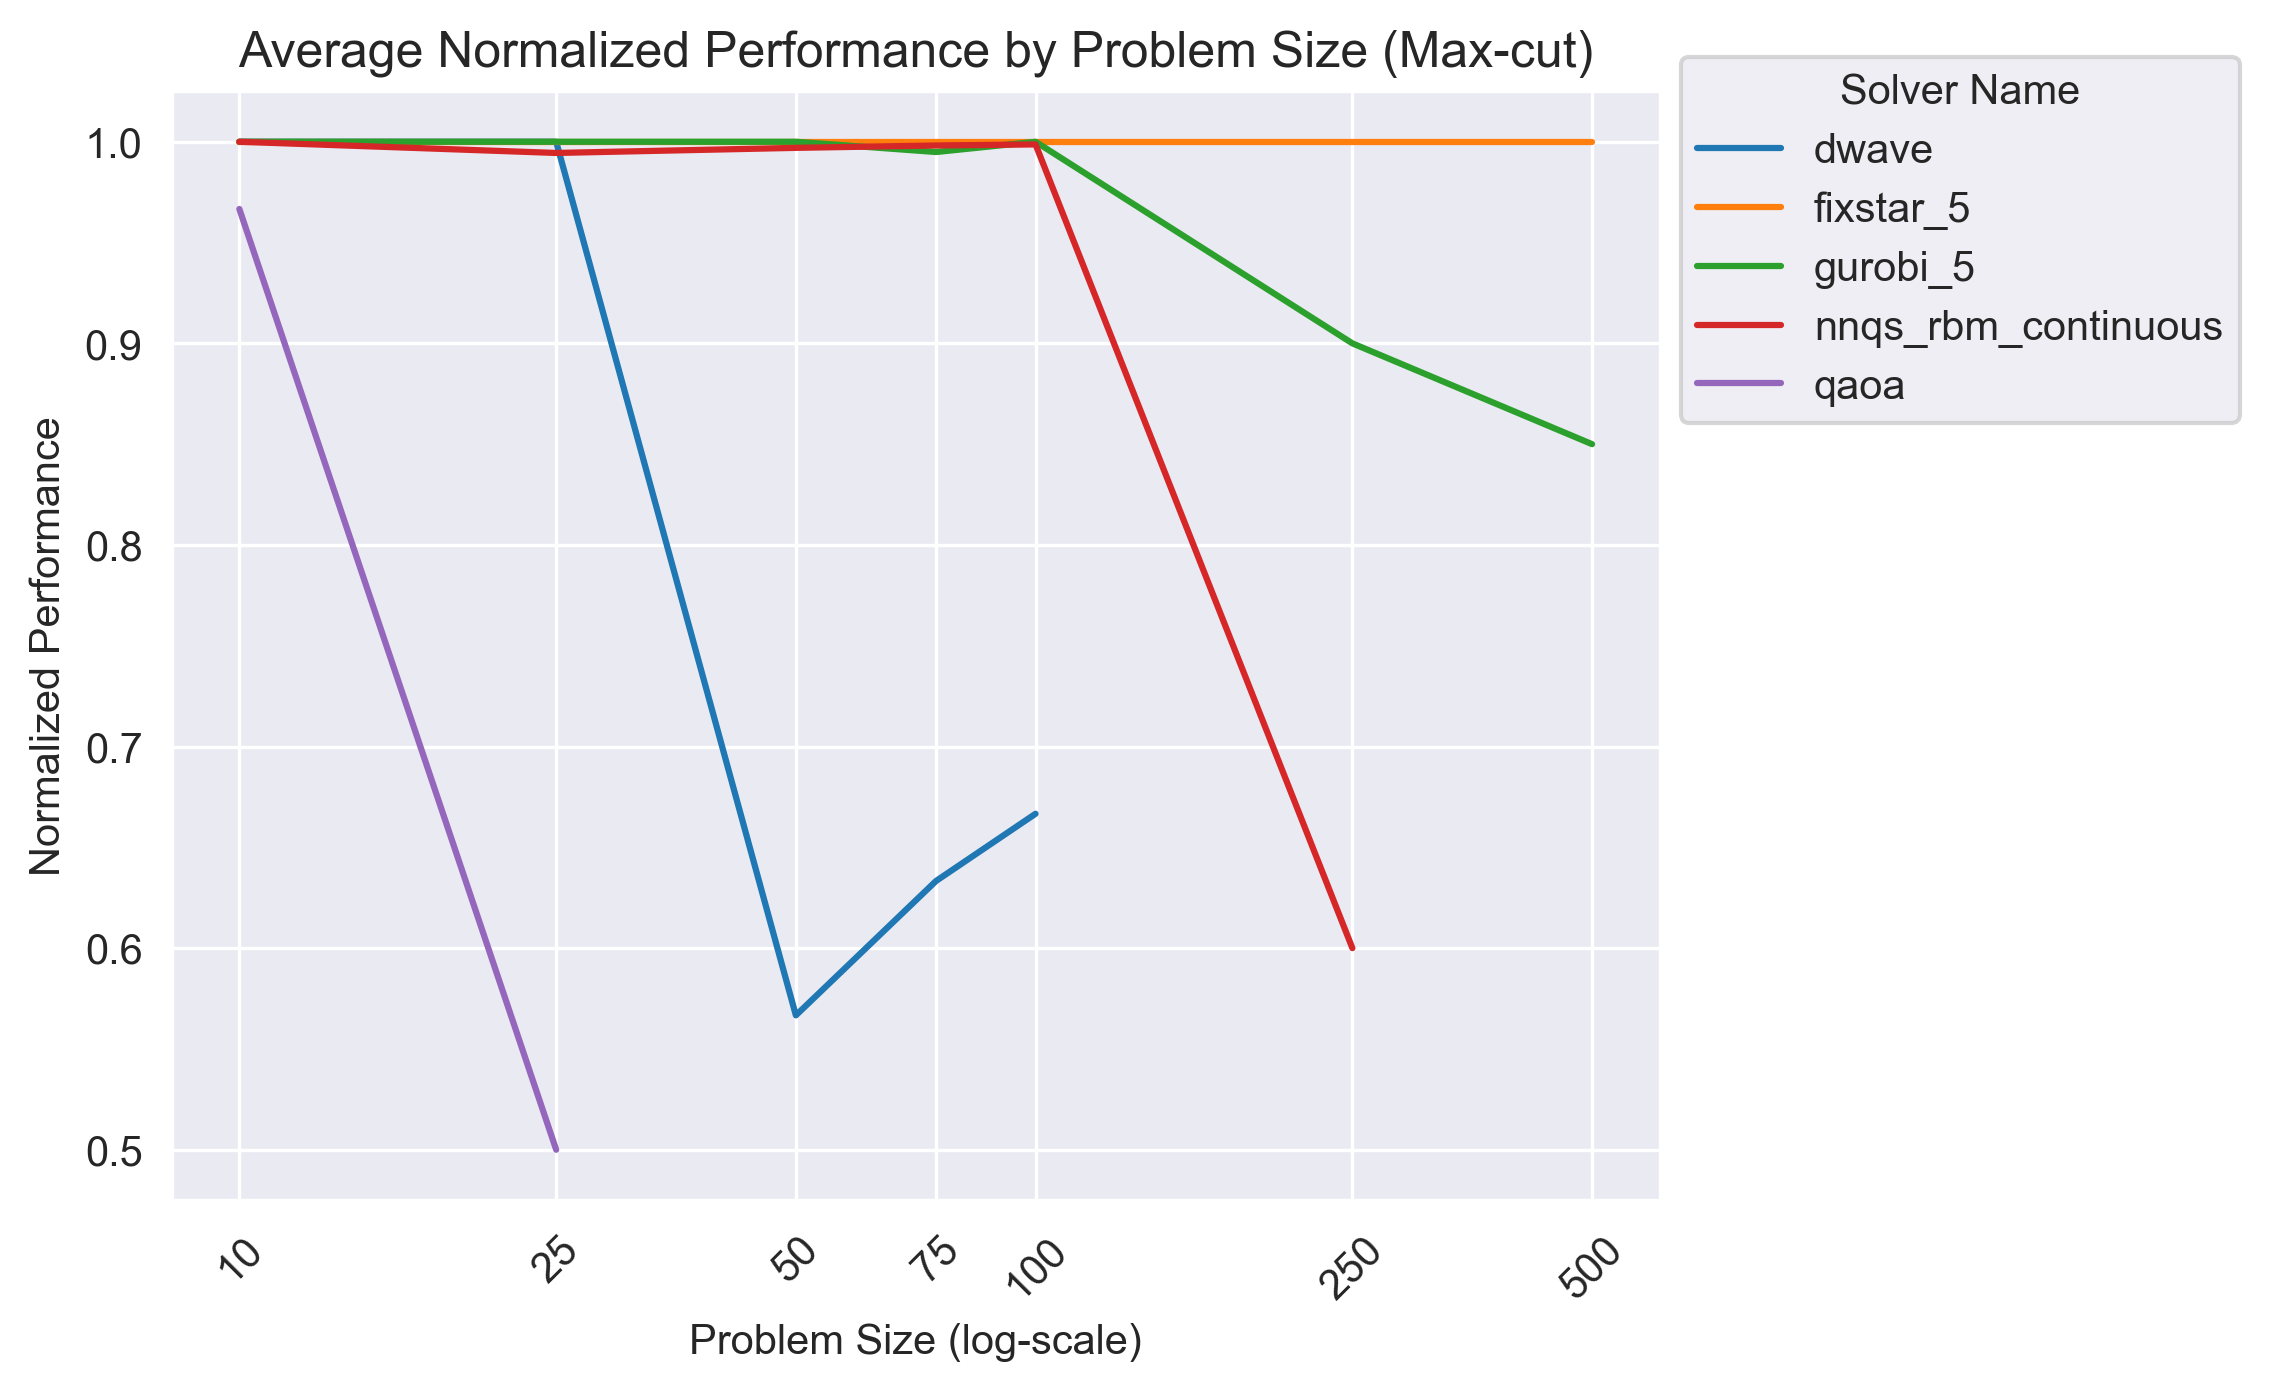
\includegraphics[width=1\linewidth]{images/maxcut_normalized_performance_all.png}
    \caption{Normalized performance by size on the max-cut dataset}
    \label{all-maxcut-size}
\end{figure}

\subsection{SK Model}
\begin{figure}[!h]
    \centering
    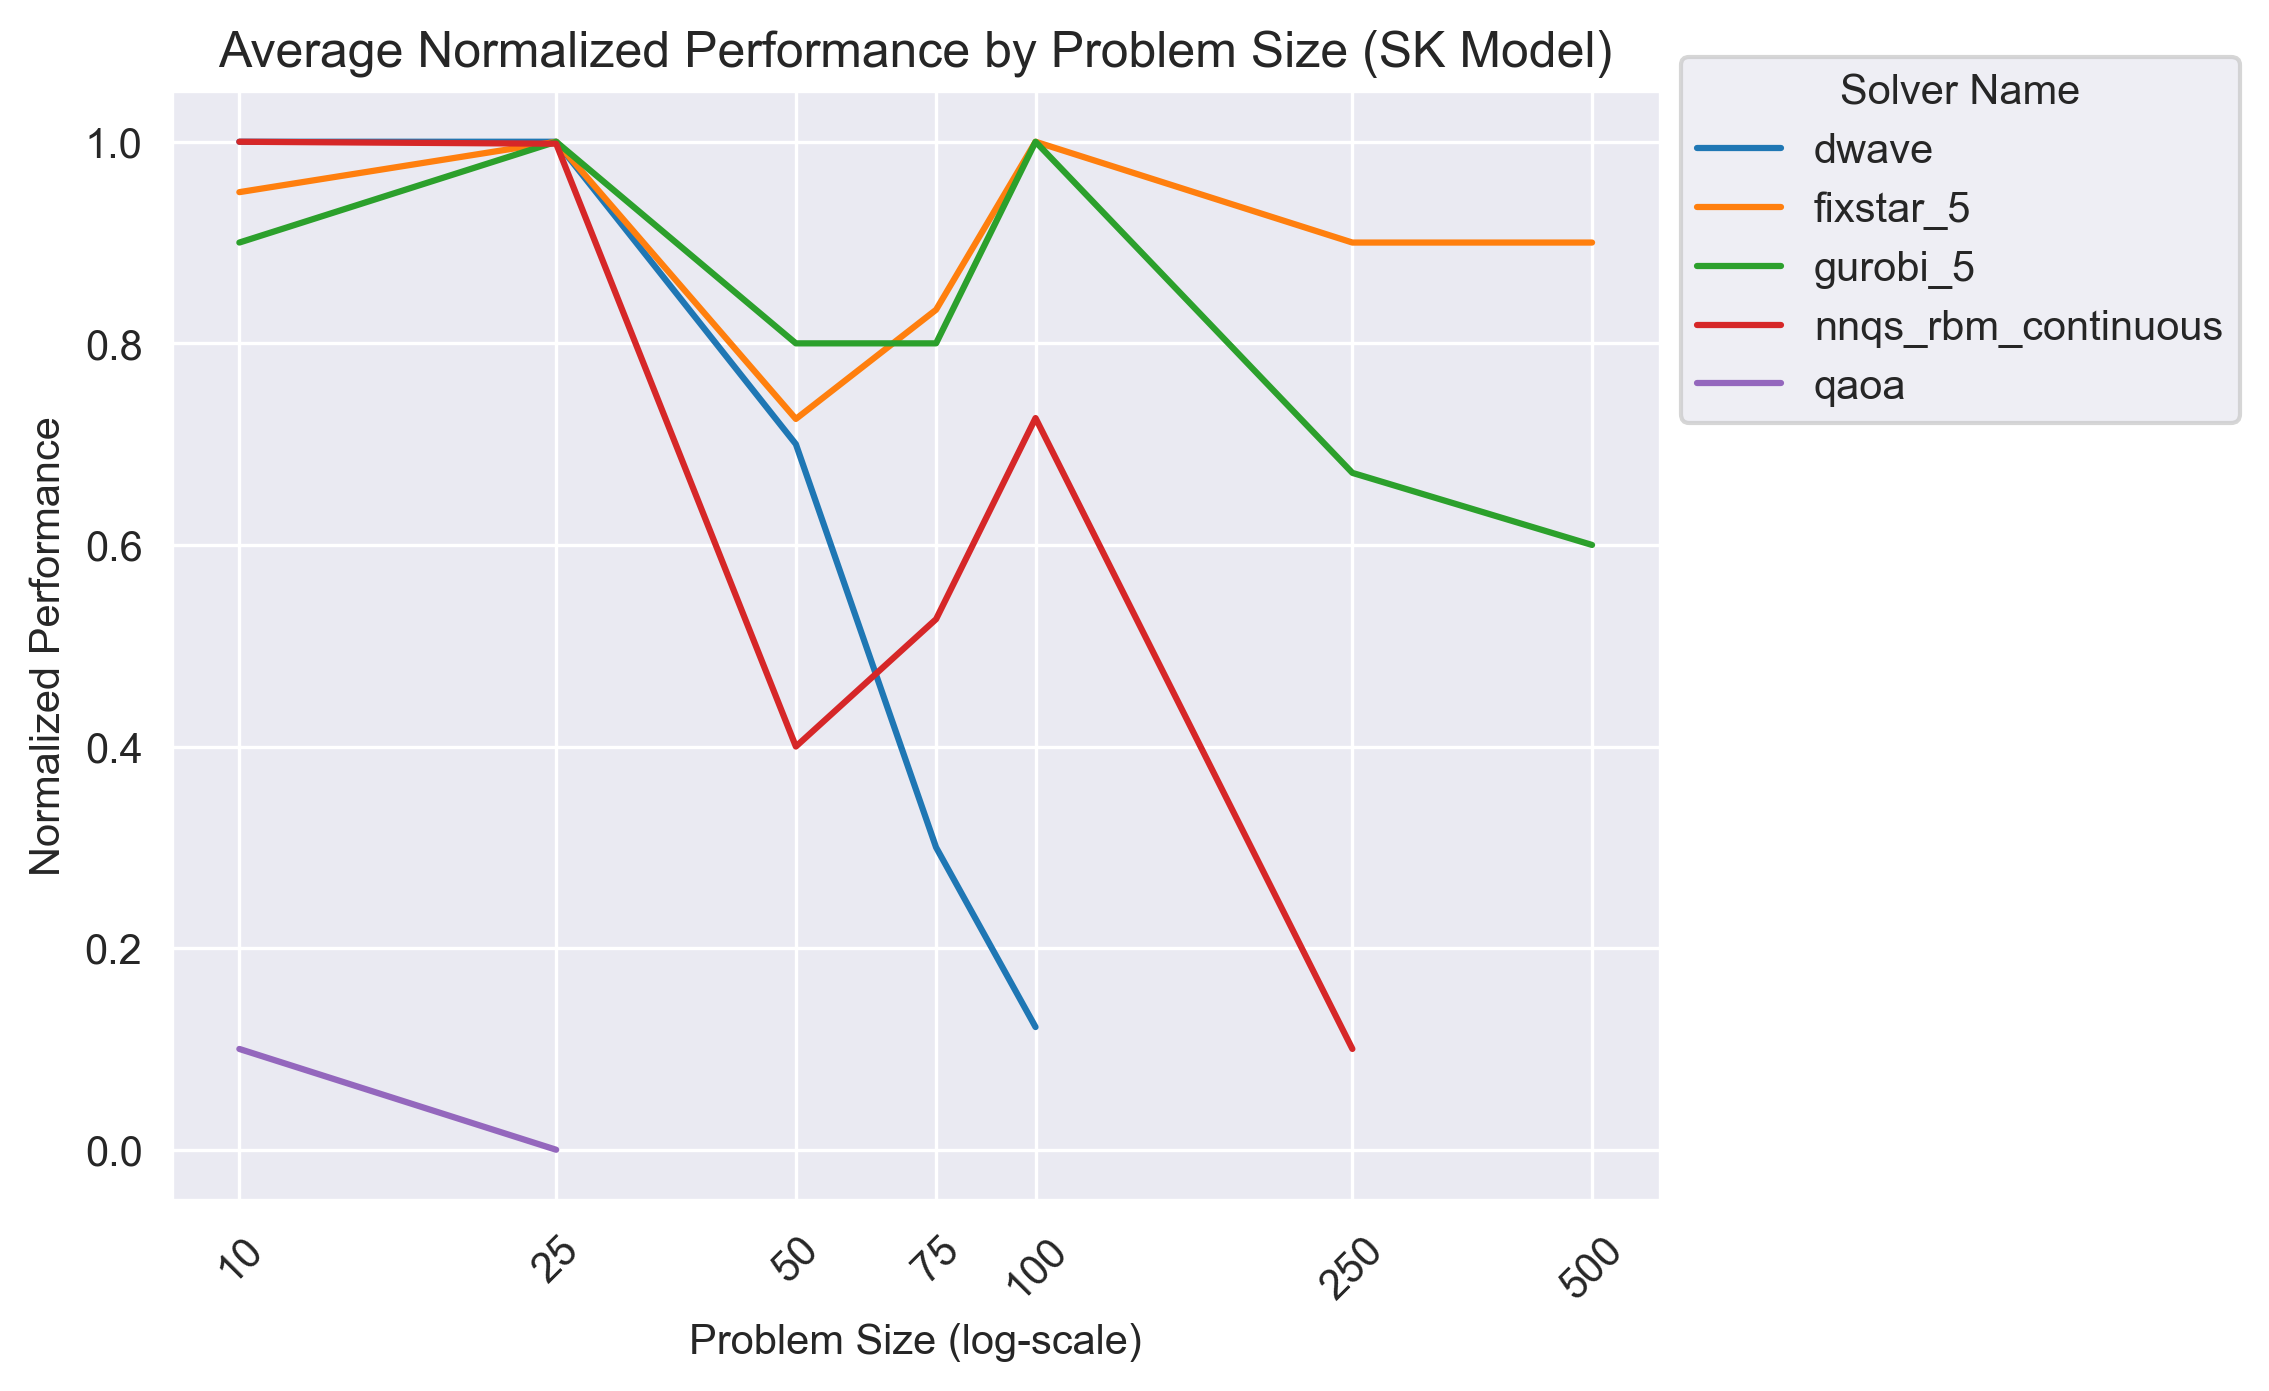
\includegraphics[width=1\linewidth]{images/skmodel_normalized_performance_all.png}
    \caption{Normalized performance by size on the SK model dataset}
    \label{all-skmodel-size}
\end{figure}